\documentclass[]{elsarticle} %review=doublespace preprint=single 5p=2 column
%%% Begin My package additions %%%%%%%%%%%%%%%%%%%
\usepackage[hyphens]{url}

  \journal{Social Science \& Medicine} % Sets Journal name


\usepackage{lineno} % add
\providecommand{\tightlist}{%
  \setlength{\itemsep}{0pt}\setlength{\parskip}{0pt}}

\usepackage{graphicx}
\usepackage{booktabs} % book-quality tables
%%%%%%%%%%%%%%%% end my additions to header

\usepackage[T1]{fontenc}
\usepackage{lmodern}
\usepackage{amssymb,amsmath}
\usepackage{ifxetex,ifluatex}
\usepackage{fixltx2e} % provides \textsubscript
% use upquote if available, for straight quotes in verbatim environments
\IfFileExists{upquote.sty}{\usepackage{upquote}}{}
\ifnum 0\ifxetex 1\fi\ifluatex 1\fi=0 % if pdftex
  \usepackage[utf8]{inputenc}
\else % if luatex or xelatex
  \usepackage{fontspec}
  \ifxetex
    \usepackage{xltxtra,xunicode}
  \fi
  \defaultfontfeatures{Mapping=tex-text,Scale=MatchLowercase}
  \newcommand{\euro}{€}
\fi
% use microtype if available
\IfFileExists{microtype.sty}{\usepackage{microtype}}{}
\bibliographystyle{elsarticle-harv}
\usepackage{graphicx}
\ifxetex
  \usepackage[setpagesize=false, % page size defined by xetex
              unicode=false, % unicode breaks when used with xetex
              xetex]{hyperref}
\else
  \usepackage[unicode=true]{hyperref}
\fi
\hypersetup{breaklinks=true,
            bookmarks=true,
            pdfauthor={},
            pdftitle={The framing of active school travel in Ontario, Canada as a health and built environment issue},
            colorlinks=false,
            urlcolor=blue,
            linkcolor=magenta,
            pdfborder={0 0 0}}
\urlstyle{same}  % don't use monospace font for urls

\setcounter{secnumdepth}{0}
% Pandoc toggle for numbering sections (defaults to be off)
\setcounter{secnumdepth}{0}

% Pandoc citation processing
\newlength{\cslhangindent}
\setlength{\cslhangindent}{1.5em}
\newlength{\csllabelwidth}
\setlength{\csllabelwidth}{3em}
% for Pandoc 2.8 to 2.10.1
\newenvironment{cslreferences}%
  {}%
  {\par}
% For Pandoc 2.11+
\newenvironment{CSLReferences}[2] % #1 hanging-ident, #2 entry spacing
 {% don't indent paragraphs
  \setlength{\parindent}{0pt}
  % turn on hanging indent if param 1 is 1
  \ifodd #1 \everypar{\setlength{\hangindent}{\cslhangindent}}\ignorespaces\fi
  % set entry spacing
  \ifnum #2 > 0
  \setlength{\parskip}{#2\baselineskip}
  \fi
 }%
 {}
\usepackage{calc}
\newcommand{\CSLBlock}[1]{#1\hfill\break}
\newcommand{\CSLLeftMargin}[1]{\parbox[t]{\csllabelwidth}{#1}}
\newcommand{\CSLRightInline}[1]{\parbox[t]{\linewidth - \csllabelwidth}{#1}\break}
\newcommand{\CSLIndent}[1]{\hspace{\cslhangindent}#1}

% Pandoc header
\usepackage{booktabs}
\usepackage{longtable}
\usepackage{array}
\usepackage{multirow}
\usepackage{wrapfig}
\usepackage{float}
\usepackage{colortbl}
\usepackage{pdflscape}
\usepackage{tabu}
\usepackage{threeparttable}
\usepackage{threeparttablex}
\usepackage[normalem]{ulem}
\usepackage{makecell}
\usepackage{xcolor}



\begin{document}
\begin{frontmatter}

  \title{The framing of active school travel in Ontario, Canada as a
health and built environment issue}
    \author[Some Department]{Author 1\corref{1}}
   \ead{author1@example.com} 
    \author[Some Department]{Author 2}
   \ead{author2@example.com} 
    \author[Another University]{Author 3\corref{2}}
   \ead{author3@example.com} 
    \author[Some Institute]{Author 4\corref{2}}
   \ead{author4@example.com} 
    \author[Some University]{Author 5}
   \ead{author5@example.com} 
    \author[Some Department]{Author 6}
   \ead{author6@example.com} 
      \address[Some Department]{Department, Street, City, Province,
Postal Code}
    \address[Another University]{Department, Street, City, Province,
Postal Code}
    \address[Some Institute]{Street, City, Province, Postal Code}
    \address[Some University]{Department, Street, City, Province, Postal
Code}
      \cortext[1]{Corresponding Author}
    \cortext[2]{Equal contribution}
  
  \begin{abstract}
  This is the abstract.

  It consists of two paragraphs.
  \end{abstract}
  
 \end{frontmatter}

\textbf{\emph{Background}}:\\
\textbf{\emph{Methods}}:\\
\textbf{\emph{Results}}: \textbf{\emph{Conclusions}}:

\newpage

\hypertarget{introduction}{%
\section{1. Introduction}\label{introduction}}

Rates of walking and bicycling to school, commonly known as active
school travel (AST), have been declining in Canada and the United States
for decades (\textbf{rothmanDeclineActiveSchool2018?}), with levels much
lower than other developed countries like The Netherlands
(\textbf{vangoeverdenSchoolTravelBehaviour2013?}), Denmark
(\textbf{jensenHowObtainHealthy2008?}), and Japan
(\textbf{waygoodChapterSixteenJapan2020?}). However, the appetite for
AST may be high in many Canadian communities. For instance, 40\% of
children in a study conducted in Toronto, Ontario who are driven to
school would like to travel by bicycle instead
(\textbf{laroucheRatherBikeSchool2016a?}). But the study reported that
less than 3\% actually do, despite the vast majority having access to a
bicycle and living within a short and bikeable distance to school.
Another study based in London, Ontario reported similar findings with
respect to children's preference for active travel
(\textbf{larsenRouteBasedAnalysisCapture2012?}). From a public health
perspective, this represents a huge opportunity to improve health and
wellbeing if more children could use active modes to school.

In response to this trend, the Government of Ontario, in Canada, created
a fund in 2017 to support communities across the province in developing
AST initiatives. Green Communities Canada runs the program, called
\emph{Ontario Active School Travel}, and determines the projects that
will be funded with their support (\textbf{GreenCommunities2016?}). As
of December 2021, OAST has funded and provided resources for over 20
projects across Ontario. Many communities implemented school travel
planning (STP), along with encouragement activities like walking school
buses or developed resources for schools and parents, among other
actions (see \textbf{GreenCommunitiesProjects?}). In this context, STP
is a popular ``school-specific'' intervention led by a facilitator that
brings together a committee of stakeholders from diverse sectors
including education, planning, transportation, and public health to
develop action plans (\textbf{buliungSchoolTravelPlanning2011?};
\textbf{mammenSchoolTravelPlanning2014?}). The five-step process
involves identifying barriers to AST based on the local context and
implementing approaches or activities following the 5 E's that alleviate
concerns about AST and make AST safer and more convenient
(\textbf{buliungSchoolTravelPlanning2011?};
\textbf{langUnderstandingModalChoice2011?}).

How AST is framed by STP stakeholders to a target audience, like parents
or the general public, may raise awareness about the issue and influence
how walking and bicycling to school are perceived. Gamson and Modigliani
(\textbf{gamsonChangingCulture1987?}) define a frame as a ``central
organizing idea or story line that provides meaning'' to a particular
phenomenon. A frame can enable individuals ``to locate, perceive,
identify, and label'' information pertaining to various dimensions of an
issue (Goffman, 1974). Therefore, stakeholder groups involved in STP
efforts can play a role in shaping public perception about AST in such a
way that it attracts greater attention and becomes a ``problem'' that
needs to be addressed through behaviour change or by new policies. We
also contend that the ways in which the AST issue is framed can affect
the policy process, as outlined in Kingdon's
(\textbf{kingdonAgendasAlternativesPublic1984?}) Multiple Streams
Framework (MSF), through all three streams (i.e., problem, policy, and
politics). This framing can ultimately impact financial contributions
and potential solutions to address the decline of AST in Canada.

After significant investment of human and financial resources to boost
rates of AST in Ontario over the past few years, we ask the following
questions: How is AST framed? What benefits of AST are communicated to
the public? What solutions are proposed to increase rates of AST? Do
proposed solutions focus primarily on the intrapersonal and
interpersonal factors, meaning that behaviour change must ultimately
result from the individual or household making different travel
decisions? Or is AST framed as an issue that must be addressed through
changes in the built environment or at the policy level?

In this paper, we use text mining and topic modelling to examine how
three STP stakeholder groups in Ontario (i.e., municipalities, school
boards, and transportation consortia) frame the issue of AST. We
assembled a corpus of texts from webpages that can be considered an
important source of information for the general public or parents who
are interested in AST. We examine word frequency, bigrams, and
concordances in these selected documents, and also identify key topics
presented by each stakeholder group. We then compare the findings from
these documents to a selection of studies on AST and explore the extent
to which there is concordance between the literature on AST and
materials shared with the public.

\hypertarget{literature-review}{%
\section{2. Literature Review}\label{literature-review}}

\hypertarget{benefits-of-active-school-travel}{%
\subsection{2.1. Benefits of active school
travel}\label{benefits-of-active-school-travel}}

The benefits of AST are valuable information to communicate to the
public in order to convey the importance of this issue. The desire to
increase AST in Canada is certainly warranted - there is compelling
evidence that children who actively commute to school earn physical and
mental health benefits. Faulkner et al. (2009) concluded from their
systematic review that children who travel on foot or by bicycle to
school generally have higher levels of physical activity than their
peers who are driven to school. However, Schoeppe et al. (2015) reported
no association between AST and physical activity. This relationship
could be dose-dependent, meaning that children would have to travel
longer distances to accumulate physical activity. A walking distance of
1000-1600 metres to school has been found to contribute to overall
levels of physical activity for boys
(\textbf{faulknerSchoolTravelChildren2013?}). The daily routine of
travelling to school can be a good opportunity for children to regularly
build physical activity into their schedule
(\textbf{mitraIndependentMobilityMode2013?}). Research has also shown
that using active modes to school contributes to improvements in
cardiovascular fitness
(\textbf{borrestadExperiencesRandomisedControlled2012?}).

More recently, there has been literature exploring the link between
transport and children's wellbeing
(\textbf{waygoodTransportChildrenWellbeing2020?}), with relevant
applications to the study of travel satisfaction (van den Berg et al.,
2020; \textbf{westmanChildrenTravelSchool2017?}). Being driven to school
reduces community interactions for children which may impact their
social wellbeing (\textbf{waygoodChildrenTravelIncidental2015?}),
whereas walking and bicycling give children opportunities to socialize
with friends or siblings
(\textbf{michailChildrenExperiencesTheir2021?}). This is something that
children highly value about travel
(\textbf{zwertsHowChildrenView2010a?}) and indicates that social
connections through travel are important for their wellbeing. AST also
provides opportunities for children to engage with the natural
environment (\textbf{fuscoUnderstandingChildrenPerceptions2012?};
\textbf{romeroChildrenExperiencesEnjoyment2015?}) which can improve
their mental or emotional wellbeing.

\hypertarget{factors-that-influence-active-school-travel-and-mode-choice}{%
\subsection{2.2. Factors that influence active school travel and mode
choice}\label{factors-that-influence-active-school-travel-and-mode-choice}}

Factors that influence AST have been presented and organized using a
socio-ecological model (SEM)
(\textbf{mitraIndependentMobilityMode2013?}) or systems model
(\textbf{badlandDevelopmentSystemsModel2016?}) whereby children's travel
behaviour is understood within the context of their household, social,
neighbourhood, and policy environments. Individual characteristics of
the child are also determinants. The SEM comes from the field of public
health and is a useful framework for understanding complex health
behaviours, including travel habits such as walking or bicycling to
school, because it identifies multiple determinants that need to be
addressed by interventions to facilitate behaviour change. The consensus
in the literature is that various factors are interrelated and that
interventions should target multiple levels in order to increase levels
of healthy and physically active modes of travel to school
(\textbf{mitraIndependentMobilityMode2013?}). Rather than describing an
extensive list of factors that influence AST and mode choice in Canada,
which has been covered elsewhere (e.g., Mammen et al., 2012; Wilson et
al., 2018; \textbf{mitraIndependentMobilityMode2013?};
\textbf{rothmanDeclineActiveSchool2018?}), we briefly discuss a few
potentially modifiable determinants that may be targeted for change
through STP.

At the individual level, older child age is often associated with AST
(Mammen et al., 2012; Wilson et al., 2018;
\textbf{starkExploringIndependentActive2018?}) as parents typically
escort younger children. There is some evidence that gender is a
determinant of AST (\textbf{larsenInfluencePhysicalEnvironment2009?}),
with boys being more likely to travel using active modes than girls,
although this is not a strong or consistent finding (Schoeppe et al.,
2015; \textbf{rothmanDeclineActiveSchool2018?}). Children's mode choice
to school is strongly influenced by their parents' travel behaviours and
the complexity of their household's travel needs (Buliung et al., 2021),
which indicates that shifting parental perceptions and habits is
important. Convenience and inclement weather have been cited by parents
as barriers to AST (\textbf{buliungSchoolTravelPlanning2011?}). Parental
perceptions of the built or school environment (De Meester et al., 2014;
Panter et al., 2010) and their children's skills (Ghekiere et al., 2017)
also influence whether they allow their children to walk or bicycle to
school.

Distance between home and school is most strongly associated with AST
(Ikeda et al., 2018; Mammen et al., 2012; Pont et al., 2009;
\textbf{rothmanDeclineActiveSchool2018?}) with less AST reported among
children who have to travel farther to school. Many studies have also
found that the quality of the built environment along the route to
school and around the school site (Ikeda et al., 2018; Kim and Lee,
2020; \textbf{rothmanActiveSchoolTransportation2021?}) and provision of
active travel infrastructure (Pont et al., 2009;
\textbf{chenPromotingActiveStudent2018a?}) facilitate AST. Canadian
youth report that they feel most safe bicycling on streets in their
neighbourhood or that have low volumes of traffic
(\textbf{TACbikeinfra2020?}). Finally, concerns about traffic and
strangers have been reported by parents who drive their children to
school (Mammen et al., 2012), which highlights that the volume and speed
of cars can be a concern or deterrent for AST.

\hypertarget{school-travel-planning-in-canada}{%
\subsection{2.3. School travel planning in
Canada}\label{school-travel-planning-in-canada}}

School travel planning (STP) has been implemented in Canada since at
least the late 2000s. Within the STP process, facilitators generally
establish multi-sector committees who intervene at the participating
school through a range of activities related to the 5E's such as
\emph{education} strategies, \emph{encouragement} through in-person
events or programs, \emph{engineering} improvements to or around the
school site, and \emph{enforcement} of traffic speeds around schools
(Mammen et al., 2014; \textbf{langUnderstandingModalChoice2011?}). The
first large-scale evaluation of STP as an intervention in Canada took
place at twelve schools across the country, including four in Ontario,
using parental surveys to measure changes in travel behaviour and
perceptions (\textbf{buliungSchoolTravelPlanning2011?}). Since then,
there have been other assessments of both the efficacy of STP
(Buttazzoni et al., 2019; Mammen et al., 2014) and the process of
implementing such programs in Ontario (Buttazzoni et al., 2018;
\textbf{mammenPuttingSchoolTravel2015?}). STP facilitators have
recommended that additional time and resources are needed to improve the
efficacy of STP (\textbf{mammenPuttingSchoolTravel2015?}), which
highlights that long-term and sustained efforts driven at the policy
level are required to address declining rates of AST.

The ways in which AST is framed seem particularly important to shift
parental attitudes and perceptions given their reported influence on
children's travel mode to school. STP activities heavily focus on
education or encouragement (Buttazzoni et al., 2018; Mammen et al.,
2014; \textbf{buliungSchoolTravelPlanning2011?}), but parents may not
always be receptive to the goals of STP and may be resistant to
behaviour change (see Buttazzoni et al., 2018). Parents have been found
to express different understandings, language, and perceptions than
planners of the built environment determinants that influence school
travel (Buliung et al., 2021). This is also true when it comes to other
factors like convenience of different modes to school
(\textbf{langUnderstandingModalChoice2011?}). STP stakeholder groups
must pay special attention to parents' understanding of the decline of
AST as a problem, which may affect their receptivity to proposed
solutions.

The ``central organizing idea or story line'' of AST, to apply the
definition from Gamson and Modigliani
(\textbf{gamsonChangingCulture1987?}), could also affect broader support
in the community. Municipal representatives are perceived to be
instrumental but the involvement of other stakeholder groups (e.g.,
busing consortium representatives and local residents) can be lacking
(Buttazzoni et al., 2018). In Ontario, it would be reasonable to say
that AST has become a policy issue on the education and public health
agendas over this time as evidenced by the financial contribution from
the provincial government. The support from a range of municipal
representatives (see Buttazzoni et al., 2018;
\textbf{mammenPuttingSchoolTravel2015?}) demonstrates that the ``policy
stream'' (see \textbf{kingdonAgendasAlternativesPublic1984?}) has been
well engaged. It is unknown to what degree the general public (i.e.,
local residents) has been exposed to messaging about AST, which could
affect their participation in the STP process as desired by STP
facilitators (Buttazzoni et al., 2018).

The success of STP interventions would likely depend on parental
judgments of factors that are related to school travel, as well as
support from key policy makers. For example, parents have been found to
view mixed land use as conducive for driving, despite transport planners
viewing neighbourhoods with mixed uses as key for encouraging more
active travel (Buliung et al., 2021). Therefore, stakeholder groups
involved in STP must make important choices about the proposed solutions
and potential benefits that ought to be communicated to parents and the
general public about AST to convey its importance as a policy issue and
to facilitate adoption of AST. Publicly available content about AST,
therefore, needs to effectively engage multiple audiences on this policy
issue including parents, children, politicians, and school
representatives. This information should reflect current knowledge from
research on school travel, plus content specific to local factors that
influence AST, so that the challenges of AST are adequately defined and
the opportunities or solutions to address the problems are clear.
However, it is unknown to what degree STP materials presented to the
general public reflect the scope of evidence from the literature on AST.

\hypertarget{data}{%
\section{3. Data}\label{data}}

\hypertarget{data-retrieval}{%
\subsection{3.1. Data retrieval}\label{data-retrieval}}

\hypertarget{policy-documents}{%
\subsubsection{3.1.1. Policy documents}\label{policy-documents}}

We assembled a collection of publicly available documents that were
sourced online from the main stakeholder groups involved in STP
initiatives in Ontario: i) school boards (public or Catholic and
English-speaking only); ii) municipal governments; and iii)
transportation consortia. The latter are a unique group of entities
sanctioned by Ontario's Ministry of Education in Ontario 2006. Each
consortium involves a collaboration between regions and school boards;
the consortium's objective is to deliver more efficient and timely
transportation services to schools in each region
(\textbf{ministryeducation2006?}). Non-profit organizations, police
services, and advocacy groups are other stakeholders who often play a
role in supporting AST and/or STP, but this study does not include any
documents from these groups because they are not consistently
participating in all initiatives across Ontario.

The search was guided first by a list of all English public and Catholic
school boards across Ontario. The websites of each school board were
manually searched for pages related to school transport or travel. Any
pages relevant to these topics were manually downloaded. Next, we
collected documents by searching municipal government and transportation
consortia websites. These were identified based on geographic area
(i.e., the municipalities and/or transportation consortia that are in
the same geographic area of each school board). Webpages related to
active transport or school travel were manually downloaded.

Webpages from STP stakeholder groups were included in our analysis if
they were easy to find. This primary criterion was important since our
analysis pertains to how such issues are framed to the general public.
Thus, we included only webpages that were readily accessible, which we
defined as requiring no more than 2-4 separate links from the initial
Google search.

The initial corpus of documents from STP stakeholder groups included 69
relevant webpages (i.e., one page or more) from all STP stakeholder
groups. We refer to these as policy documents throughout the paper. It
is important to note that school boards, municipalities, and
transportation consortia may or may not publish information about their
involvement in AST and STP efforts on their respective websites or in
policy documents. Search results are summarized in Table
\ref{tab:policy-documents}.

\begin{table}

\caption{\label{tab:policy-documents}\label{tab:search-results}Search results from the main STP stakeholder groups.}
\centering
\resizebox{\linewidth}{!}{
\begin{tabular}[t]{>{}l|l|>{}l}
\toprule
Stakeholder & Total & Included\\
\midrule
\cellcolor{gray!6}{\textbf{School boards}} & \cellcolor{gray!6}{62} & \cellcolor{gray!6}{32}\\
\textbf{Municipalities} & 62 & 28\\
\cellcolor{gray!6}{\textbf{Transportation consortia}} & \cellcolor{gray!6}{39} & \cellcolor{gray!6}{9}\\
\bottomrule
\end{tabular}}
\end{table}

\hypertarget{academic-papers}{%
\subsubsection{3.1.2. Academic papers}\label{academic-papers}}

\textbf{To be completed by Dr.~Paez}

\hypertarget{data-cleaning}{%
\subsection{3.2. Data cleaning}\label{data-cleaning}}

A multi-step process was conducted to ensure that the analysis captured
as much text as possible from both the policy documents (n = 64) and
academic papers (n = 233). To begin, the webpages, which were manually
downloaded in portable document format (PDF), were trimmed so that pages
that only consisted of tables, figures, or references were removed. Many
academic papers were in a two-column format, which is not ideal for
conversion to \texttt{txt}. We adapted a procedure
(https://stackoverflow.com/questions/42541849/extract-text-from-two-column-pdf-with-r)
to read the two-column PDF documents so that they would be converted
correctly. Four academic papers did not join sufficiently and were taken
out of the corpus due to the substantial time required to manually
correct their inconsistencies.

Next, we converted the trimmed PDF documents into \texttt{txt} files so
that they could be imported in R for analysis. We then proceeded to a
manual cleaning phase where we removed any remaining tables, figures,
references, headers/footings, and captions that could not be trimmed.
Manual corrections were also required for certain pages in academic
papers that remained in two-column format after the conversion process.
This typically occurred on pages that had a table or figure which
disrupted the text. Finally, we reviewed all of the documents to remove
hyphenation by line breaks and to keep hyphenated words together on the
same line. Any ligatures (e.g., combinations of characters or letters
that were not properly detected during the conversion process) were
fixed by replacing the unicode sequence of character by inserting the
missing sequence of characters.

We also manually removed any extraneous material in the academic papers
that did not pertain to AST specifically. This included footnotes,
references, acknowledgments, and conflict of interest statements in the
academic papers. We removed all phone numbers, inserted links to other
webpages, personal names, and content not to specific to AST from the
policy documents that were retrieved from the websites of school boards,
municipalities, and transportation consortia.

In the final step, we removed all blank spaces, punctuation,
capitalization, and numbers. English stop words, which are common words
such as \emph{and} or \emph{the} as identified in a predetermined list
by Lewis et al. (\textbf{R-tm?}) and other frequent terms in the
documents like ``school'' and specific location names, were removed from
the corpora.

\hypertarget{methods}{%
\section{4. Methods}\label{methods}}

\hypertarget{framing-analysis}{%
\subsection{4.1. Framing analysis}\label{framing-analysis}}

Issues that pertain to public health or wellbeing are often presented to
the public through particular frames to influence perceptions or
behaviours. As previously mentioned, a frame is a ``central organizing
idea or story line that provides meaning'' to a public issue or
phenomenon (\textbf{gamsonChangingCulture1987?}). Scholars in the field
of political communications have proposed that communicators, such as
the media or an institution, construct the narrative of a frame for
policy positions or public issues in order to activate or restrict a
particular response in the intended audience (Pan and Kosicki, 1993).
Organized groups of stakeholders can employ similar methods to attract
attention to particular issues. Framing can be used to position existing
solutions as suitable to address particular issues (Mah et al., 2014),
which may prevent the public from being aware of other policy approaches
that challenge the status quo. The way policy issues are framed is
ultimately important to understand because it plays a role in either
altering or preserving the existing social perceptions. This, in turn,
can affect whether issues are put on the agenda of policy makers and can
determine which solutions are proposed to address the problem
(\textbf{kingdonAgendasAlternativesPublic1984?}).

Framing of issues is an important step in developing health policy. An
obvious example over the past decade is the framing of climate change as
a public health issue (e.g., Depoux et al., 2017; Maibach et al., 2010;
Weathers and Kendall, 2016) to increase public engagement and awareness
of the issue. This framing has slowly advanced this issue on public
policy agendas as public attention puts pressure on the policy stream to
adopt frameworks for action. For example, transport planners also use
different frames to guide the extent to which transport policies can be
adapted to address climate change. In a recent paper
(\textbf{reynardGrowthResilienceHow2021?}), framing analysis was applied
to review the representation of issues such as mobility and social
exclusion in municipal policies from four western Canadian cities under
the current circumstances of climate change. The authors found four
primary frames: ``The Growing City,'' ``If You Build It, They Will
Come,'' ``Better City for All,'' and a ``the Resilient City''
(\textbf{reynardGrowthResilienceHow2021?}). Each frame presented the
nature, opportunities, and challenges of climate change in different
ways which set the stage for the types of mitigation and adaptation
strategies that cities were proposing to address this issue.

In a similar way, we hypothesize that STP stakeholder groups in Ontario
have framed AST in particular ways to effectively engage multiple
audiences on this policy issue including parents, local residents,
school representatives, and municipal representatives. These groups are
likely identifying points of intervention and potential opportunities to
build support for and encourage AST.

\hypertarget{topic-modelling}{%
\subsection{4.2. Topic modelling}\label{topic-modelling}}

We use topic modelling in R to conduct the framing analysis. Topic
modelling is a machine learning technique that can identify what
language and concepts are being communicated by analyzing text. This
method is more practical for researchers working with large amounts of
text because it replaces the manual coding of topics that would normally
take place to analyze or summarize textual data
(\textbf{jacobiQuantitativeAnalysisLarge2016?}). In the data
pre-processing phase, we tokenize the text in the documents and create a
document-term matrix so that it is in the correct format for analysis.
We primarily use the following packages: \texttt{tidytext}
(\textbf{R-tidytext?}), \texttt{topicmodels} (\textbf{R-topicmodels?}),
\texttt{word2vec} (\textbf{R-word2vec?}), and \texttt{wordcloud}
(\textbf{R-wordcloud?}) to examine text in the documents that were
sourced for this project. These packages have functions for determining
the frequency of specific words in each document or relationships (e.g.,
pairs of adjacent terms called bigrams) and correlations between words.
These methods can reveal what language and concepts are being
communicated to the general public. Topic modelling is a popular method
for analyzing text from social media platforms
(\textbf{albalawiUsingTopicModeling2020?}) or news articles
(\textbf{jacobiQuantitativeAnalysisLarge2016?}). We estimate latent
Dirichlet allocation (LDA) models to classify both the STP and documents
according to the topics that are contained within them. This method
``treats each document as a mixture of topics, and each topic as a
mixture of words'' (\textbf{silgeTextMining2021?}). The model's output
is ``a set of topics consisting of clusters of words that co-occur in
these documents according to certain patterns''
(\textbf{jacobiQuantitativeAnalysisLarge2016?}). Researchers must then
interpret the identified topics, as done after other methods of manual
coding. We also compare the topics between the policy documents and the
academic papers, and use our interpretation to answer the questions
outlined above that guide this paper. This methodology is not familiar
to many, so we describe in more detail below how we used specific
functions and code in R to produce our results.

\hypertarget{reproducibility}{%
\subsection{4.3. Reproducibility}\label{reproducibility}}

This paper is an example of open and reproducible research that uses
only open software. All data were obtained from publicly available
sources and organized in the form of a data package. Following best
practices in spatial data science (\textbf{brunsdon2020opening?}), the
code and data needed to reproduce or conduct a similar analysis for
other regions in North America or elsewhere are available for download.

\hypertarget{results}{%
\section{5. Results}\label{results}}

\hypertarget{word-and-document-frequency}{%
\subsection{5.1. Word and document
frequency}\label{word-and-document-frequency}}

We analyzed word and document frequency for each set of documents (i.e.,
corpus). Table \ref{tab:word-table} shows the most frequent terms found
in the municipal, transportation consortia, school board, and academic
documents. As expected, policy documents and academic papers reference
\emph{active travel}, \emph{walking}, \emph{biking} or \emph{cycling},
and \emph{students} more than other terms. Each corpus also has
\emph{safety} and \emph{traffic} as common words which suggests
congruence on these key factors between the research literature and how
AST is framed to the public. The word \emph{physical} is present in each
corpus, but it's not clear what this refers to (e.g, \emph{physical
activity}, \emph{physical health}, or the \emph{physical environment}).
Furthermore, documents from STP stakeholder groups discuss
\emph{resources}, \emph{information}, and \emph{services} about school
travel. In the section below, the context in which these terms are
discussed is explored further.

Unlike the academic papers, policy documents include the words
\emph{route} or \emph{routes} as frequent terms. This could reflect the
role of STP stakeholder groups in identifying safe routes to school to
share with parents or families, as well as the STP emphasis on making
the physical environment safer for AST. The academic corpus differs from
the policy documents in that \emph{parents} and \emph{distance} are the
second and third most common terms. In addition, \emph{time},
\emph{factors}, \emph{environment}, and \emph{age} are also identified
in the academic papers. These words are absent from the list of common
words in policy documents. Table \ref{tab:word-table} indicates that the
academic corpus discusses a broader range of determinants of AST than
the policy documents. The number of references for each term in the
academic papers is also significantly higher due to the inclusion of
more documents.

\begin{table}

\caption{\label{tab:word-table}\label{tab:word-table}Top 25 terms identified in each corpora. Document frequencies are also indicated.}
\centering
\resizebox{\linewidth}{!}{
\begin{tabular}[t]{lcclcclcclcc}
\toprule
\multicolumn{3}{c}{Municipalities} & \multicolumn{3}{c}{School Boards} & \multicolumn{3}{c}{Transportation Consortia} & \multicolumn{3}{c}{Academic Papers} \\
\cmidrule(l{3pt}r{3pt}){1-3} \cmidrule(l{3pt}r{3pt}){4-6} \cmidrule(l{3pt}r{3pt}){7-9} \cmidrule(l{3pt}r{3pt}){10-12}
Term & Count (n) & Documents (n) & Term & Count (n) & Documents (n) & Term & Count (n) & Documents (n) & Term & Count (n) & Documents (n)\\
\midrule
\cellcolor{gray!6}{active} & \cellcolor{gray!6}{248} & \cellcolor{gray!6}{26} & \cellcolor{gray!6}{active} & \cellcolor{gray!6}{124} & \cellcolor{gray!6}{13} & \cellcolor{gray!6}{active} & \cellcolor{gray!6}{67} & \cellcolor{gray!6}{7} & \cellcolor{gray!6}{walking} & \cellcolor{gray!6}{5137} & \cellcolor{gray!6}{222}\\
travel & 126 & 20 & bus & 120 & 20 & walking & 55 & 8 & parents & 3946 & 211\\
\cellcolor{gray!6}{walking} & \cellcolor{gray!6}{90} & \cellcolor{gray!6}{25} & \cellcolor{gray!6}{travel} & \cellcolor{gray!6}{103} & \cellcolor{gray!6}{11} & \cellcolor{gray!6}{walk} & \cellcolor{gray!6}{49} & \cellcolor{gray!6}{8} & \cellcolor{gray!6}{distance} & \cellcolor{gray!6}{3271} & \cellcolor{gray!6}{205}\\
bike & 87 & 15 & information & 65 & 21 & travel & 41 & 8 & students & 2960 & 173\\
\cellcolor{gray!6}{cycling} & \cellcolor{gray!6}{78} & \cellcolor{gray!6}{22} & \cellcolor{gray!6}{walking} & \cellcolor{gray!6}{57} & \cellcolor{gray!6}{17} & \cellcolor{gray!6}{students} & \cellcolor{gray!6}{39} & \cellcolor{gray!6}{9} & \cellcolor{gray!6}{cycling} & \cellcolor{gray!6}{2753} & \cellcolor{gray!6}{171}\\
\addlinespace
safety & 71 & 21 & walk & 53 & 13 & safety & 32 & 6 & environment & 2631 & 202\\
\cellcolor{gray!6}{health} & \cellcolor{gray!6}{65} & \cellcolor{gray!6}{21} & \cellcolor{gray!6}{weather} & \cellcolor{gray!6}{40} & \cellcolor{gray!6}{11} & \cellcolor{gray!6}{help} & \cellcolor{gray!6}{29} & \cellcolor{gray!6}{9} & \cellcolor{gray!6}{activity} & \cellcolor{gray!6}{2371} & \cellcolor{gray!6}{209}\\
physical & 63 & 18 & safety & 40 & 19 & schools & 25 & 9 & traffic & 2353 & 208\\
\cellcolor{gray!6}{traffic} & \cellcolor{gray!6}{59} & \cellcolor{gray!6}{20} & \cellcolor{gray!6}{safe} & \cellcolor{gray!6}{39} & \cellcolor{gray!6}{19} & \cellcolor{gray!6}{children} & \cellcolor{gray!6}{25} & \cellcolor{gray!6}{6} & \cellcolor{gray!6}{choice} & \cellcolor{gray!6}{2299} & \cellcolor{gray!6}{169}\\
road & 56 & 13 & services & 37 & 17 & community & 24 & 7 & physical & 2256 & 215\\
\addlinespace
\cellcolor{gray!6}{activity} & \cellcolor{gray!6}{55} & \cellcolor{gray!6}{14} & \cellcolor{gray!6}{planning} & \cellcolor{gray!6}{37} & \cellcolor{gray!6}{7} & \cellcolor{gray!6}{bus} & \cellcolor{gray!6}{18} & \cellcolor{gray!6}{4} & \cellcolor{gray!6}{trips} & \cellcolor{gray!6}{2194} & \cellcolor{gray!6}{170}\\
schools & 52 & 14 & parents & 32 & 17 & route & 17 & 5 & car & 2148 & 195\\
\cellcolor{gray!6}{children} & \cellcolor{gray!6}{47} & \cellcolor{gray!6}{15} & \cellcolor{gray!6}{sustainable} & \cellcolor{gray!6}{31} & \cellcolor{gray!6}{8} & \cellcolor{gray!6}{zone} & \cellcolor{gray!6}{16} & \cellcolor{gray!6}{6} & \cellcolor{gray!6}{safety} & \cellcolor{gray!6}{2140} & \cellcolor{gray!6}{204}\\
plan & 45 & 16 & children & 31 & 14 & resources & 16 & 6 & time & 2101 & 218\\
\cellcolor{gray!6}{students} & \cellcolor{gray!6}{44} & \cellcolor{gray!6}{14} & \cellcolor{gray!6}{child} & \cellcolor{gray!6}{31} & \cellcolor{gray!6}{12} & \cellcolor{gray!6}{day} & \cellcolor{gray!6}{16} & \cellcolor{gray!6}{4} & \cellcolor{gray!6}{factors} & \cellcolor{gray!6}{2101} & \cellcolor{gray!6}{216}\\
\addlinespace
walk & 43 & 18 & day & 29 & 13 & safe & 15 & 5 & child & 2085 & 187\\
\cellcolor{gray!6}{public} & \cellcolor{gray!6}{39} & \cellcolor{gray!6}{15} & \cellcolor{gray!6}{routes} & \cellcolor{gray!6}{28} & \cellcolor{gray!6}{14} & \cellcolor{gray!6}{planning} & \cellcolor{gray!6}{15} & \cellcolor{gray!6}{4} & \cellcolor{gray!6}{walk} & \cellcolor{gray!6}{2008} & \cellcolor{gray!6}{200}\\
community & 37 & 19 & physical & 28 & 11 & physical & 15 & 7 & public & 1983 & 208\\
\cellcolor{gray!6}{safe} & \cellcolor{gray!6}{34} & \cellcolor{gray!6}{16} & \cellcolor{gray!6}{health} & \cellcolor{gray!6}{28} & \cellcolor{gray!6}{11} & \cellcolor{gray!6}{healthy} & \cellcolor{gray!6}{14} & \cellcolor{gray!6}{6} & \cellcolor{gray!6}{age} & \cellcolor{gray!6}{1783} & \cellcolor{gray!6}{211}\\
benefits & 32 & 17 & inclement & 25 & 11 & traffic & 13 & 6 & urban & 1768 & 200\\
\addlinespace
\cellcolor{gray!6}{play} & \cellcolor{gray!6}{31} & \cellcolor{gray!6}{2} & \cellcolor{gray!6}{eligibility} & \cellcolor{gray!6}{24} & \cellcolor{gray!6}{11} & \cellcolor{gray!6}{support} & \cellcolor{gray!6}{13} & \cellcolor{gray!6}{6} & \cellcolor{gray!6}{home} & \cellcolor{gray!6}{1715} & \cellcolor{gray!6}{199}\\
resources & 30 & 13 & consortium & 24 & 9 & families & 13 & 5 & social & 1713 & 191\\
\cellcolor{gray!6}{healthy} & \cellcolor{gray!6}{29} & \cellcolor{gray!6}{16} & \cellcolor{gray!6}{region} & \cellcolor{gray!6}{23} & \cellcolor{gray!6}{10} & \cellcolor{gray!6}{way} & \cellcolor{gray!6}{12} & \cellcolor{gray!6}{5} & \cellcolor{gray!6}{different} & \cellcolor{gray!6}{1713} & \cellcolor{gray!6}{215}\\
routes & 27 & 13 & service & 22 & 11 & student & 12 & 5 & mobility & 1659 & 138\\
\cellcolor{gray!6}{lanes} & \cellcolor{gray!6}{26} & \cellcolor{gray!6}{3} & \cellcolor{gray!6}{•} & \cellcolor{gray!6}{21} & \cellcolor{gray!6}{1} & \cellcolor{gray!6}{region} & \cellcolor{gray!6}{12} & \cellcolor{gray!6}{4} & \cellcolor{gray!6}{significant} & \cellcolor{gray!6}{1650} & \cellcolor{gray!6}{208}\\
\bottomrule
\multicolumn{12}{l}{\rule{0pt}{1em}\textit{Note: }}\\
\multicolumn{12}{l}{\rule{0pt}{1em} }\\
\multicolumn{12}{l}{\rule{0pt}{1em}\textsuperscript{a} Count (n) refers to the total number of times the term is found in the corpora}\\
\multicolumn{12}{l}{\rule{0pt}{1em}\textsuperscript{b} Documents (n) refers to the total number of documents that feature the term}\\
\end{tabular}}
\end{table}

\hypertarget{bigrams-and-concordances}{%
\subsection{5.2. Bigrams and
concordances}\label{bigrams-and-concordances}}

Bigrams refer to a pair of consecutive words. We use the
\texttt{unnest\_tokens} function from the \emph{tidytext} package to
determine the bigrams. Figures \ref{fig:city-visual},
\ref{fig:consortia-visual}, and \ref{fig:school-visual} show the bigrams
that occur more than 5 times for each set of policy documents. These
figures help to make further sense of the word frequencies reported
above, and highlight the main ideas that are presented to the public in
each of the policy corpora. Municipalities primarily discuss
\emph{physical activity} (n = 53) and \emph{public health} (n = 19) in
the context of AST. In addition, \emph{travel planning} (n = 19),
\emph{bike lanes} (n = 16), and \emph{safe routes} (n = 14) are also
identified, conceivably as either proposed solutions or built
environment factors that support AST. Key issues related to transport
such as \emph{traffic safety} (n = 10), \emph{air quality} (n = 9), and
\emph{greenhouse gases} (n = 9) are conveyed to the public through these
policy documents. It is not surprising to find this focus given that
municipalities in Ontario are concerned about climate change and have
increasingly looked to active modes of travel to offset
transport-related emissions in urban areas.

Similar word bigrams are found in school board documents: \emph{travel
planning} (n = 33), \emph{safe routes} (n = 15), \emph{physical
activity} (n = 10), and \emph{public health} (n = 10) are among the most
common bigrams. Both municipalities and school boards in Ontario seem to
emphasize what can be or has been done to improve AST (i.e., policy or
planning changes), while outlining some of the benefits of AST at the
individual- or community-level to potentially encourage behaviour change
(i.e., physical activity for children or improved air quality). Unlike
other STP stakeholders, school boards also consider \emph{inclement
weather} (n = 24) and \emph{bus cancellations} (n = 13). This is likely
because many students in Ontario travel to school by bus and this
information is presented alongside AST options. Finally, transportation
consortia documents highlight topics such as \emph{physical activity} (n
= 10), \emph{pedestrian safety} (n = 8), \emph{crossing guards} (n = 6),
\emph{travel planning} (n = 6), and \emph{walk zones} (n = 6). Biking or
cycling is notably absent from transportation consortia documents.
Overall, the policy documents There appears convey an emphasis on the
built environment, rather than household decision-making.

\begin{figure}

{\centering 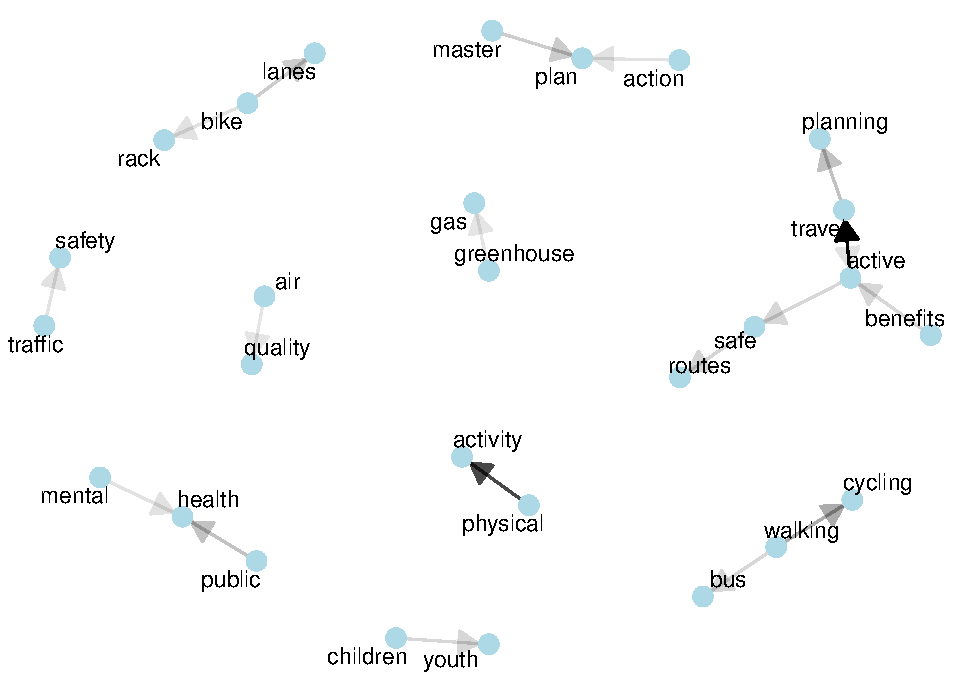
\includegraphics[width=1\linewidth]{AST-Framing-Ontario_files/figure-latex/city-visual-1} 

}

\caption{\label{fig:city-visual}Most common bigrams found in the municipal or regional government documents.}\label{fig:city-visual}
\end{figure}

\begin{figure}

{\centering 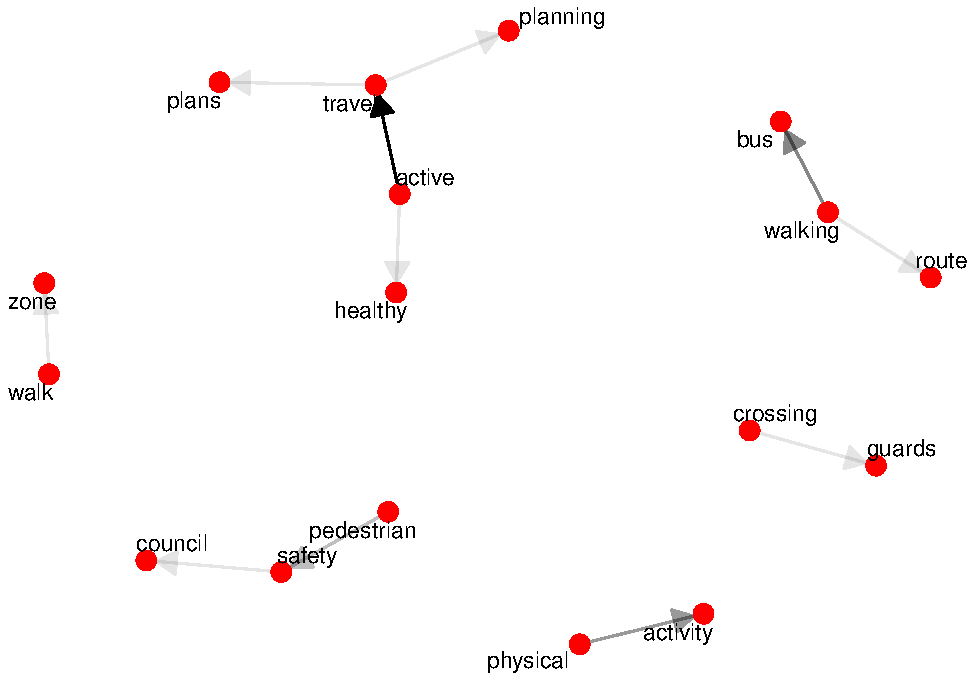
\includegraphics[width=1\linewidth]{AST-Framing-Ontario_files/figure-latex/consortia-visual-1} 

}

\caption{\label{fig:consortia-visual}Most common bigrams found in the transportation consortia documents.}\label{fig:consortia-visual}
\end{figure}

\begin{figure}

{\centering 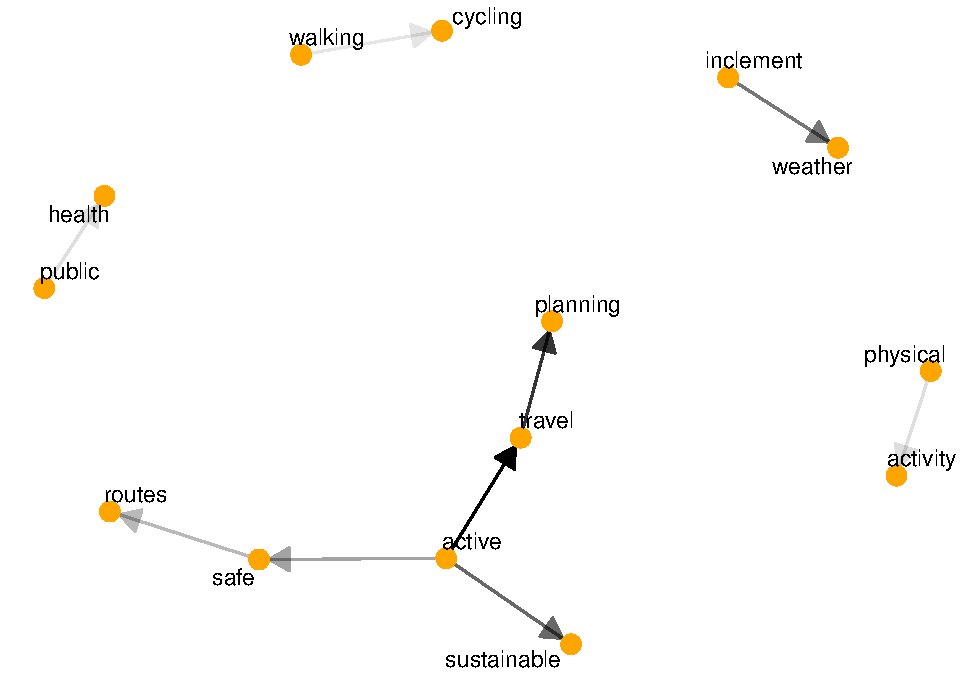
\includegraphics[width=1\linewidth]{AST-Framing-Ontario_files/figure-latex/school-visual-1} 

}

\caption{\label{fig:school-visual}Most common bigrams found in the school board documents.}\label{fig:school-visual}
\end{figure}

\begin{figure}

{\centering 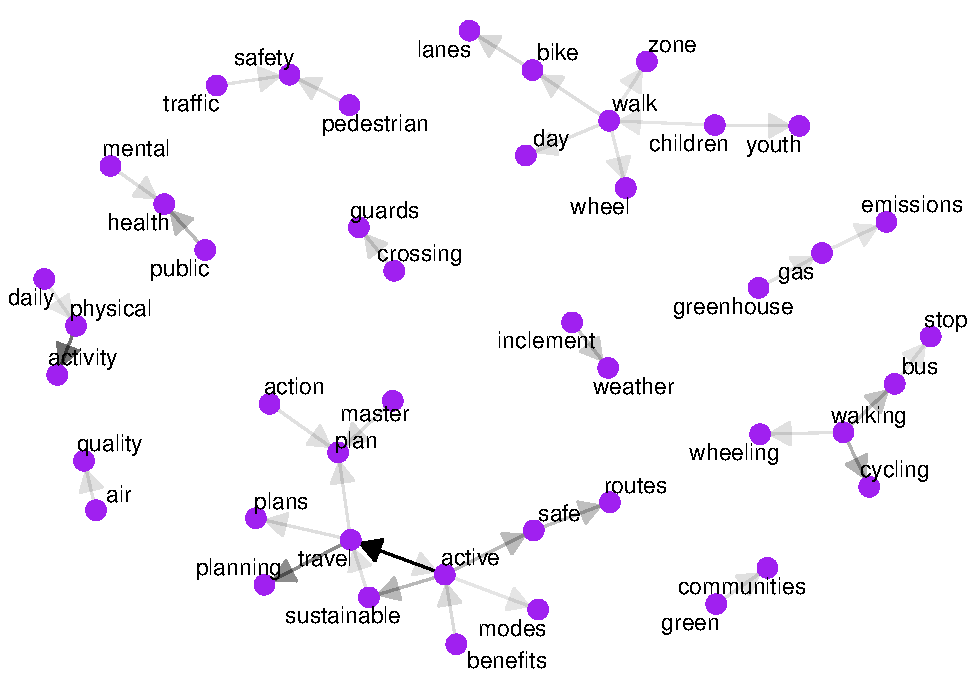
\includegraphics[width=1\linewidth]{AST-Framing-Ontario_files/figure-latex/policy-visual-1} 

}

\caption{\label{fig:policy-visual}Most common bigrams found across all policy documents (i.e., school board, municipality, and transportation consortia combined).}\label{fig:policy-visual}
\end{figure}

We then combine all municipality, school board, and transportation
consortia documents into one ``policy'' corpus. This enabled us to
examine and visualize the most common bigrams found across all of the
material in Ontario that was collected for this study. Figure
\ref{fig:policy-visual} shows all of the bigrams that occur more than 10
times in the policy corpus. In addition to the bigrams already
identified above, we also found \emph{mental health}, \emph{walk day},
and \emph{green communities} as common pairs of consecutive words. The
latter terms represent the significant involvement of the non-profit
organization in supporting AST initiatives through the Ontario Active
School Travel program. Overall, the policy documents from STP
stakeholder groups seem to focus on four key areas: i) benefits or
impacts of AST; ii) mechanisms of intervention; iii) concerns or
considerations; and iv) supports for AST. This interpretation indicates
that the general public accessing information about AST in Ontario is
informed about an adequate range of content related to this issue.

Next, we analyze bigrams in the academic corpus separately to make
comparisons with the policy corpus. Figure \ref{fig:academic-visual}
indicates that academic papers include several common bigrams that were
also found in the policy documents including \emph{physical activity} (n
= 1566), which is the top bigram, \emph{traffic safety} (n = 308), and
\emph{safe routes} (n = 268). However, many other factors are identified
in the research literature that are not presented to the general public
through policy documents. After \emph{physical activity}, \emph{built
environment} (n = 1175), \emph{independent mobility} (n = 774), and
\emph{urban form} (n = 352) are the most frequent pairs of consecutive
words. Academic papers also often discuss \emph{distance home} (n =
258), \emph{car ownership} (n = 254), \emph{household income} (n = 254),
and \emph{population density} (n = 205), which are factors that have
been found to influence AST. It is evident that many papers investigate
gender differences in AST given that \emph{boys girls} (n = 211) is
another common bigram. Finally, the presence of \emph{statistically
significant} among the top bigrams underscores that some researchers aim
to identify determinants using statistical measures. We find that the
academic corpus focuses on a greater range of topics than found in the
policy documents.

\begin{figure}

{\centering 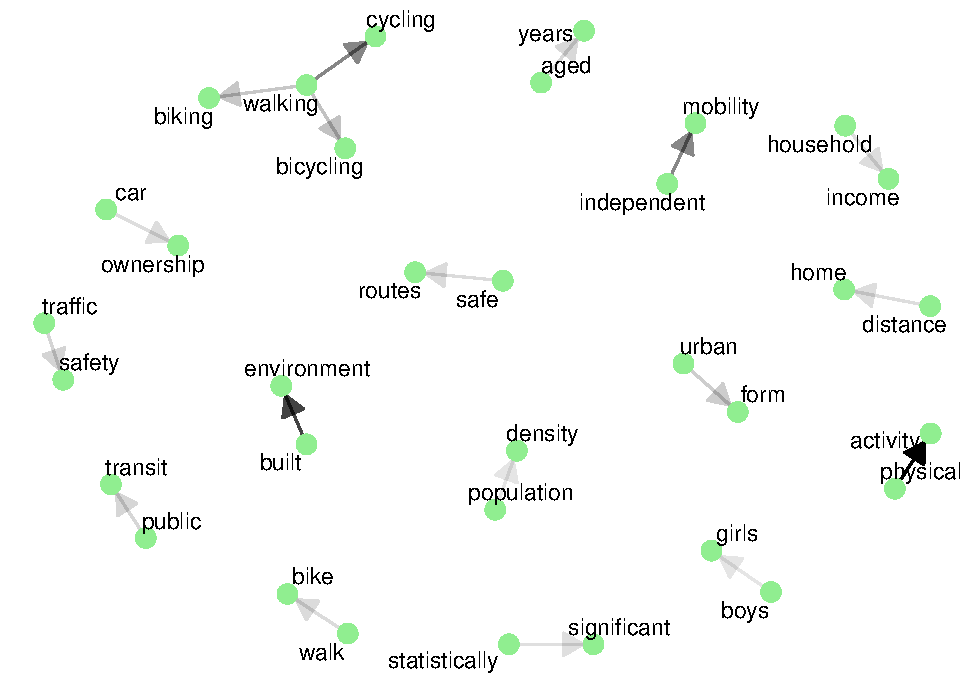
\includegraphics[width=1\linewidth]{AST-Framing-Ontario_files/figure-latex/academic-visual-1} 

}

\caption{\label{fig:academic-visual}Most common bigrams found in the academic papers.}\label{fig:academic-visual}
\end{figure}

We interpret the most common bigrams from the policy corpus (see Figure
\ref{fig:policy-visual}), which includes all documents from
municipalities, transportation consortia, and school boards, as the main
ideas that STP stakeholder groups are focusing on and communicating to
the public about AST. We then use the \texttt{kwic} function from the
\emph{quanteda} package to better understand the context of these key
ideas. Table \ref{tab:policy-concordance} presents some examples of the
context that was extracted from select policy documents to demonstrate
how the most common bigrams are communicated to the public.

\begin{table}

\caption{\label{tab:content-table}\label{tab:policy-concordance}CAPTION THIS TABLE}
\centering
\begin{tabular}[t]{>{}ll>{\raggedright\arraybackslash}p{20em}}
\toprule
Terms & Stakeholder & Context\\
\midrule
\textbf{\cellcolor{gray!6}{Air Quality}} & \cellcolor{gray!6}{School Board} & \cellcolor{gray!6}{Active transportation [...] improves air quality.}\\
\textbf{Benefit} & Municipality & Stronger bones and muscles, improved self-esteem and sense of well-being while reducing stress and risk of chronic disease all benefit those who use active transportation.\\
\textbf{\cellcolor{gray!6}{Walking School Bus}} & \cellcolor{gray!6}{School Board} & \cellcolor{gray!6}{While taking part in a walking school bus, your child will enjoy seeing friends on the way to school. They will be active more often. This is also a great opportunity for your child to socialize with school friends in a monitored and safe way where they can practice social distancing, modelled by a leader.}\\
\textbf{Community} & School Board & Help your students get started on the right foot - encourage them to walk or bike to school when possible. Even leaving the car a block or two and walking the rest of the way helps. It’s good for the environment and your health, and teaches your child independence and community awareness.\\
\textbf{\cellcolor{gray!6}{Emissions}} & \cellcolor{gray!6}{Consortia} & \cellcolor{gray!6}{An active school commute also reduces congestion in school zones and contributes to reducing greenhouse gas emissions – it’s a win-win for everyone!}\\
\addlinespace
\textbf{Health} & Municipality & Active School Travel allows school-aged children the chance to participate in moderate to intense physical activity. This is linked with lower body mass index and improved cardiovascular health.\\
\textbf{\cellcolor{gray!6}{Lanes}} & \cellcolor{gray!6}{Municipality} & \cellcolor{gray!6}{We are continuing to build on the cycling and pedestrian network by adding more bike lanes, building multi-use paths and encouraging developments to provide better pedestrian/cycling environments.}\\
\textbf{Mental Health} & Municipality & ASST not only improves physical and mental health but contributes to a healthier environment and safer streets.\\
\textbf{\cellcolor{gray!6}{Physical Health}} & \cellcolor{gray!6}{Municipality} & \cellcolor{gray!6}{Encouraging Active Transportation promotes personal health and recreation, helps manage congestion, reduces emissions and supports municipal objectives for efficient land use.}\\
\bottomrule
\end{tabular}
\end{table}

\hypertarget{topic-modelling-1}{%
\subsection{5.3. Topic modelling}\label{topic-modelling-1}}

\begin{verbatim}
## Warning: `guides(<scale> = FALSE)` is deprecated. Please use `guides(<scale> =
## "none")` instead.
\end{verbatim}

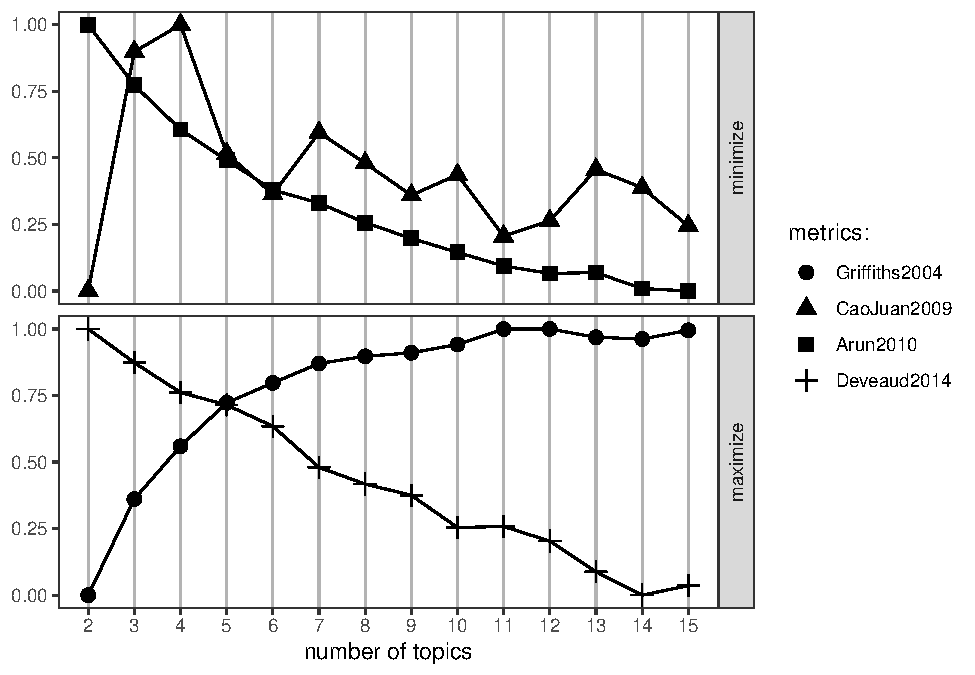
\includegraphics{AST-Framing-Ontario_files/figure-latex/evaluate-lda-1.pdf}

\begin{verbatim}
## Warning: `guides(<scale> = FALSE)` is deprecated. Please use `guides(<scale> =
## "none")` instead.
\end{verbatim}

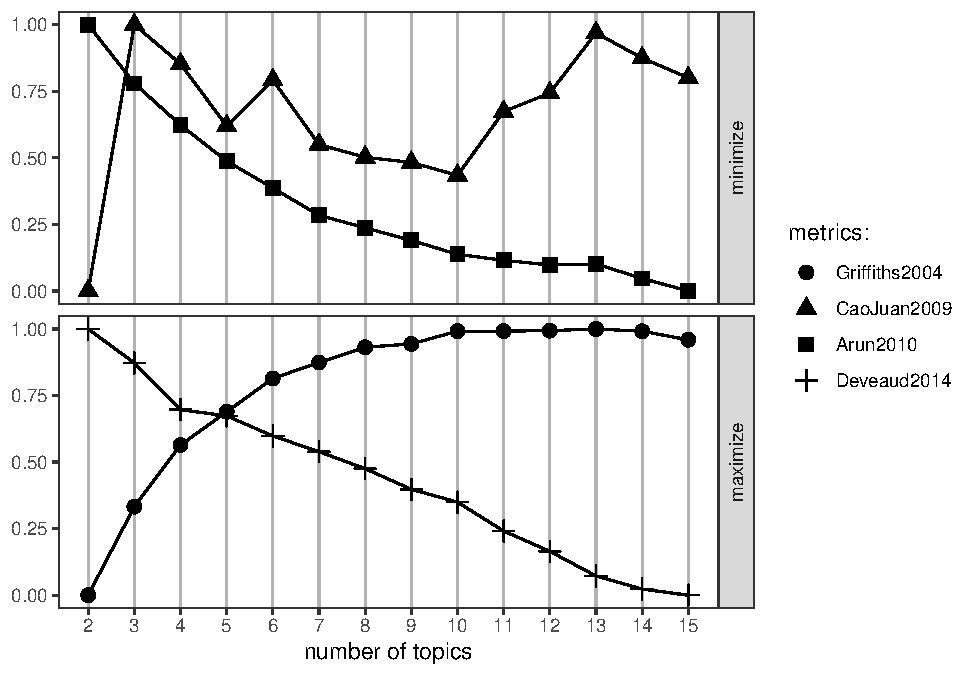
\includegraphics{AST-Framing-Ontario_files/figure-latex/evaluate-lda-2.pdf}

\begin{verbatim}
## Warning: `guides(<scale> = FALSE)` is deprecated. Please use `guides(<scale> =
## "none")` instead.
\end{verbatim}

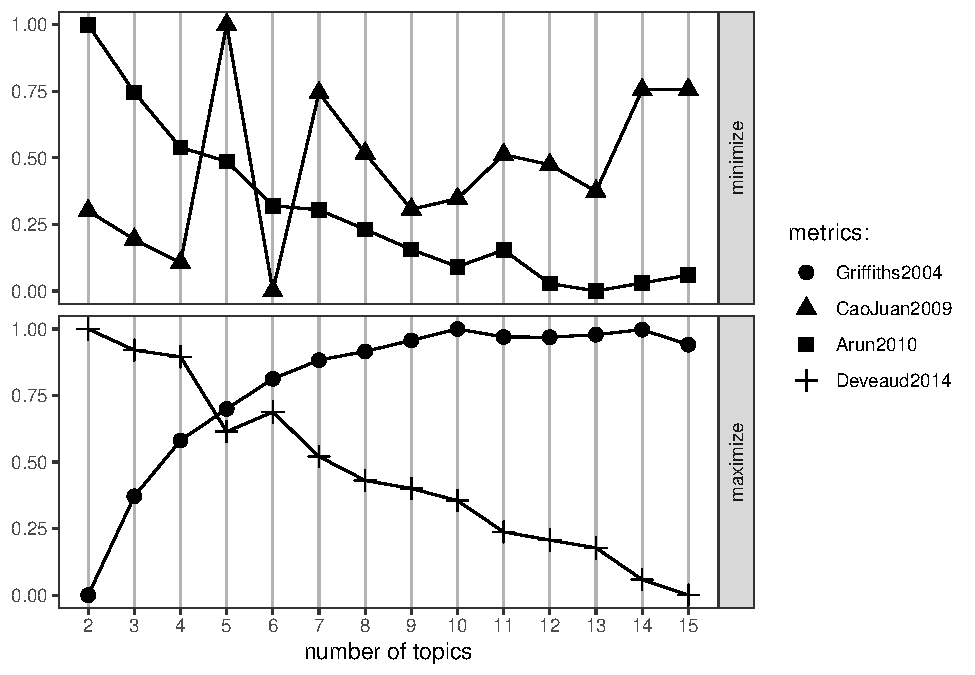
\includegraphics{AST-Framing-Ontario_files/figure-latex/evaluate-lda-3.pdf}

\begin{verbatim}
## Warning: `guides(<scale> = FALSE)` is deprecated. Please use `guides(<scale> =
## "none")` instead.
\end{verbatim}

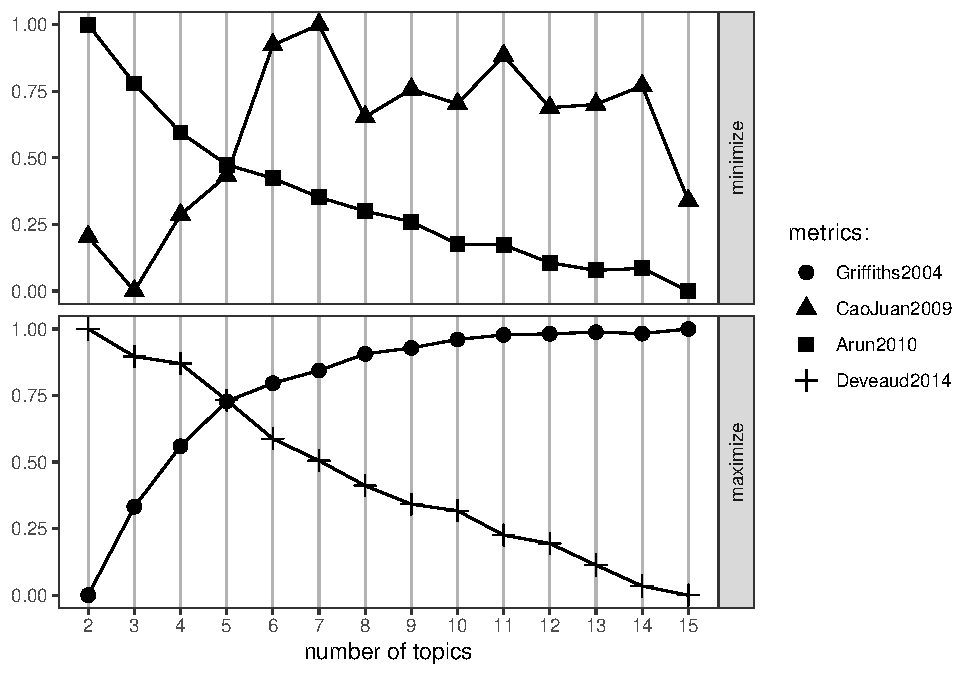
\includegraphics{AST-Framing-Ontario_files/figure-latex/evaluate-lda-4.pdf}

\begin{figure}
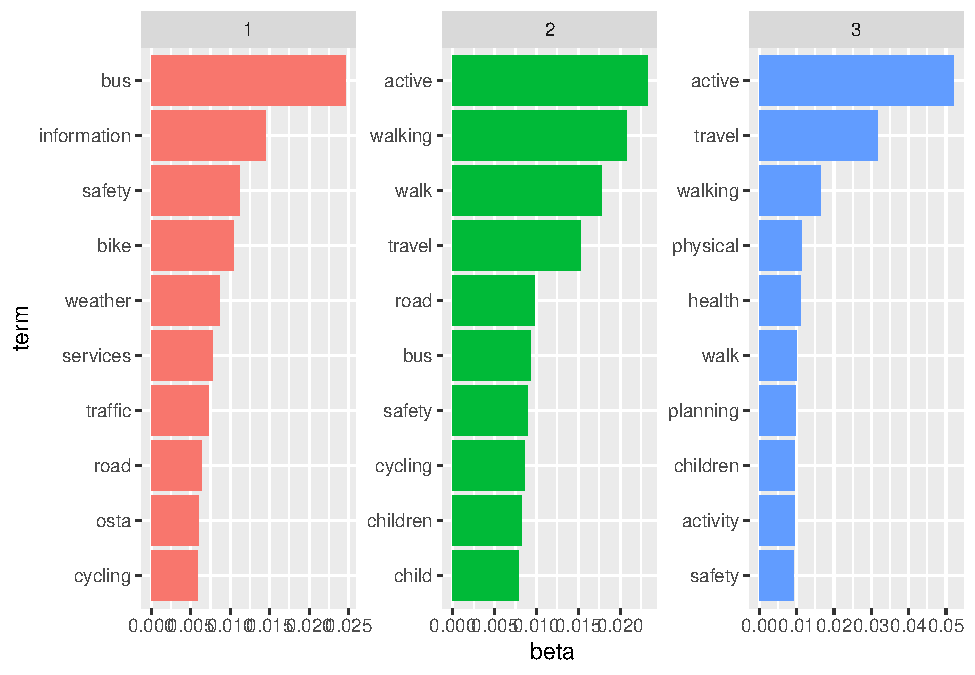
\includegraphics[width=1\linewidth]{AST-Framing-Ontario_files/figure-latex/policy-terms-1} \caption{\label{fig:policy-terms}CAPTION THIS FIGURE}\label{fig:policy-terms}
\end{figure}

\begin{figure}
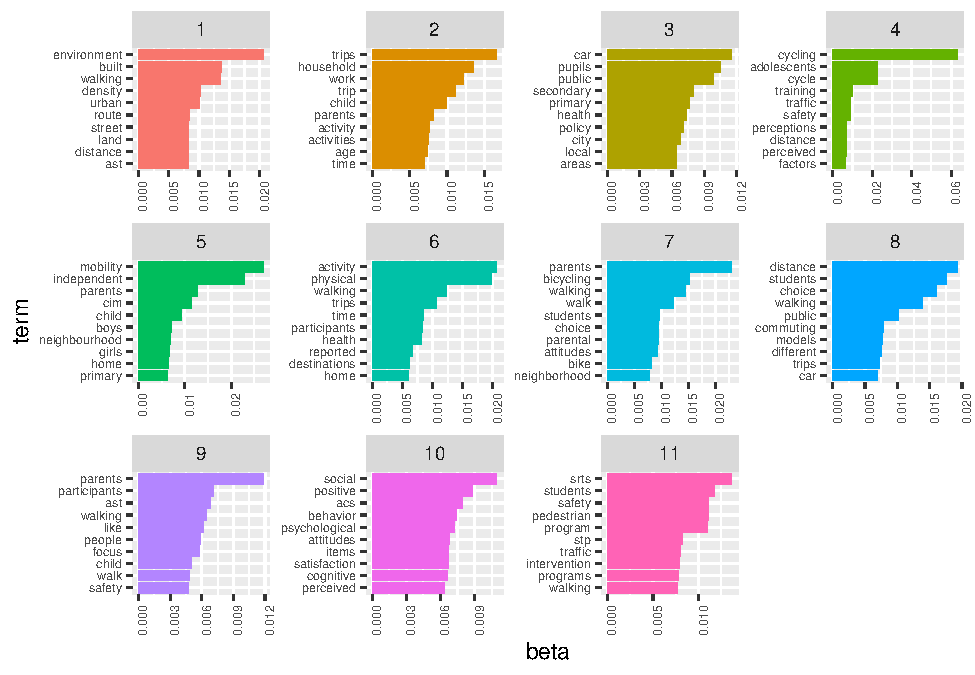
\includegraphics[width=1\linewidth]{AST-Framing-Ontario_files/figure-latex/academic-terms-1} \caption{\label{fig:academic-terms}CAPTION THIS FIGURE}\label{fig:academic-terms}
\end{figure}

Finally, we conduct topic modelling to examine the different topics
found in the policy and academic corpora. We focus on the policy corpus,
instead of individually assessing the municipal, school, and consortia
documents, so that we could report on the various frames used across all
documents put out by STP stakeholder groups in Ontario. To determine the
number of discrete topics in each corpus, we use the \emph{ldatuning}
package. We then use the \texttt{LDA} function from the
\emph{topicmodels} package to estimate an LDA model for each group of
documents. The parameters from the \emph{ldatuning} package suggest that
the policy corpus has between 7 and 9 topics and the academic corpus has
between 17 and 25 topics. After running the LDA model for the academic
corpus, it was too difficult to interpret a minimum of 17 topics based
on the clusters of words that were identified. We experimented with the
model by adjusting the number of topics and found that there were 9
distinct topics that could be interpreted, after which there was too
much overlap. Figures \ref{fig:policy-terms} and
\ref{fig:academic-terms} present the main terms that are associated with
the topics found in each corpus.

In the policy corpus, we interpret the following topics based on the
cluster of words: (1) resources for walking, (2) busing information and
eligibility; (3) benefits of active travel; (4) bicycling and the
environment; and (5) supporting active travel. These topics indicate
that STP stakeholder groups are sending the message that walking and
bicycling to school are healthy travel modes for students, particularly
as a means to get physical activity. We also found that there is
information shared to support parents and students in using active modes
to school such as the availability of cycling lanes or route tips for
walking.

The academic corpus has a higher number of topics likely due to the
volume of papers that were sourced. The following topics were identified
based on the clusters of words: (1) \textbf{unclear} (2) AST in Ontario
and Canada; (3) \textbf{unclear}; (4) children's independent mobility;
(5) safe routes to school programs; (6) commuting and distance; (7)
density in the built environment and walking routes; (8)
\textbf{unclear}; (9) walking interventions; (10) bicycling influences;
(11) interpersonal and household influences on trips; (12) behaviours
and attitudes; (13) \textbf{unclear}; (14) \textbf{unclear}; (15)
walking distance; (16) \textbf{unclear}; (17) physical activity measures
or results; (18) bicycling attitudes; and (19) \textbf{unclear}.

We conclude that the policy corpus primarily frames AST as a health and
environmental issue. Policy documents do not reflect the diversity of
content found in the academic papers and instead focus on a few factors.
STP stakeholder groups appear to position walking, bicycling, or rolling
to school as beneficial to individual health, as an opportunity for
physical activity or to improve mental health, and to the broader
community through a reduction in traffic and vehicle emissions. Here, we
present some examples from the policy documents to illustrate how the
health and environmental frames are communicated:

\begin{quote}
\emph{If you live in a walk zone, the best way to get to school is by
walking or biking. This promotes physical activity, helps the
environment and minimizes traffic around schools during busy times.}
(City of Barrie)
\end{quote}

\begin{quote}
\emph{Walking to school is a great way to add physical activity into
your child's busy day.} (Region of Haldimand-Norfolk Region)
\end{quote}

\begin{quote}
\emph{Active school travel is a great way for children to be physically
active, which is associated with improved physical and mental health,
while making school zones safer, by reducing traffic volumes at and
around schools.}(Region of Leeds, Grenville and Lanark)
\end{quote}

\begin{quote}
\emph{The WCDSB supports active transportation as the preferred method
of transportation to school because it is a healthy choice that has
proven links to greater student achievement.} (Waterloo Catholic
District School Board)
\end{quote}

However by examining document frequency (see Section 5.1), we found that
some terms are not present in all policy documents. This suggests that
although documents pertain to the subject of active travel or school
travel, some stakeholders across Ontario are not disseminating
information about AST. For example, a document may discuss active travel
but not to school or school travel but only by bus and not by active
modes. We manually searched the policy corpus and found that 48\% of
documents mention AST and 16\% mention STP. This confirms that many
municipalities, school boards, and transportation consortia are not
promoting AST through their webpages or indicating their involvement in
the STP process. Instead, inclement weather and impacts to busing is a
common topic addressed in school board and transportation consortia
documents.

Furthermore, we found that some policy documents make direct reference
to topics found in the academic papers. For example, some policy
documents encourage AST programs that have been researched and evaluated
in the literature, such as walking school buses, or explain how an
increase in AST will reduce parent safety concerns.

\begin{quote}
\_ For their health, safety, environment and community: Kids learn
healthy habits and concentrate better in class; One less car (yours)
reduces traffic and parking problems in school zones; Teach your kids
about traffic safety; Start a walking school bus; your kids make friends
in every grade, and that can prevent bullying.\_ (City of Guelph)
\end{quote}

\begin{quote}
\emph{There are lots of benefits in the classroom for children that walk
or cycle to school on a regular basis. Some of these benefits include
improved concentration and better coping with stress. Being outside
helps to prevent feelings of isolation and increases their social
interactions. Walking and biking to school can also save you money and
lead to fewer cars on the road.} (City of Ottawa)
\end{quote}

The secondary frame for AST in policy documents is the opportunity or
prospect of behaviour change. Some cities and schools explain how
children and parents can leave the car at home and make the journey to
school on foot or by bike by describing efforts to make AST safer. This
frame encourages the public to evaluate their own travel decisions and
to access resources (e.g., walking skills checklist) that will help them
make AST a first choice. Some documents emphasize the role of the parent
in creating opportunities for AST in their household or neighbourhood,
however few documents address the main barriers as perceived by parents
(e.g., distance, travel arrangements for multiple people, or
convenience). Examples of this secondary frame include:

\begin{quote}
\_A way to make sure your child is safe while walking to school is with
a `walking school bus.' Here are some tips for a walking school bus:
Invite families who live nearby to walk; Pick a route and take a test
walk; Take side streets and paths that are less busy with traffic;
Decide how often the group will walk together; Talk with your boss to
adjust your day; Have fun! (City of Ottawa)
\end{quote}

\begin{quote}
Help your students get started on the right foot - encourage them to
walk or bike to school when possible. Even leaving the car a block or
two and walking the rest of the way helps. It's good for the environment
and your health, and teaches your child independence and community
awareness.\_ (Halton District School Board)
\end{quote}

\begin{quote}
\emph{Want to boost your child's mental and physical health? Ottawa
Public Health, City of Ottawa, and OSTA have produced a tipsheet for
parents about ``active transportation'' to school -- fitting walking and
wheeling into your daily routine.} (Ottawa-Carleton District School
Board)
\end{quote}

Finally, the policy documents discuss proposed solutions to encourage
AST. STP stakeholder groups seem to be communicating that AST is
possible and safe as a result of improvements to the built environment
and available resources for parents and children. A final focus in the
policy documents is on various efforts that are underway to support
active travel including route planning.

\begin{quote}
\emph{School Travel Planning is a community-based approach that aims to
increase the number of students and adults choosing active and
sustainable travel to get to and from school. This approach addresses
concerns about safety, physical activity, and the environment.} (City of
Hamilton)
\end{quote}

\begin{quote}
\emph{Today, as more and more of our neighbourhoods are being
retrofitted with new sidewalks and bike lanes, pedestrian crossovers,
street lights, reduced speed limits and/or crossing guards, the walk or
bike ride to and from school has never been easier, safer or healthier.}
(Hamilton-Wentworth District Catholic School Board)
\end{quote}

\hypertarget{discussion}{%
\section{6. Discussion}\label{discussion}}

\hypertarget{framing-in-stp-documents}{%
\subsection{6.1. Framing in STP
documents}\label{framing-in-stp-documents}}

Using topic modelling, we analyzed how AST is framed in documents
available to the general public on the websites of STP stakeholder
groups in Ontario. We found that AST is primarily framed as beneficial
to the health and wellbeing of children and to environmental
sustainability. This was confirmed by the most common bigrams identified
in the policy corpus, as well as the topics identified by the LDA model.
The policy documents adequately reflect the evidence that AST
contributes positively to children's physical health (see Faulkner et
al., 2009; Schoeppe et al., 2015). STP stakeholder groups also
communicate that increasing AST may reduce traffic near and around
schools which could alleviate parental concerns about traffic safety.
The potential outcomes of increased AST are highlighted which may be
persuasive arguments to motivate behaviour change, which is the
secondary frame of AST that we interpreted based on the LDA models.

The proposed solutions to the problem of declining AST that are
communicated to the general public are mostly educational (e.g., safety
tips or maps of safe routes) and engineering changes (e.g., traffic
calming or bicycle lanes). These solutions have to sufficiently address
real and perceived concerns that pose barriers to AST in order to
encourage adoption. In most documents, the emphasis is on providing
parents with resources that help them switch modes for the school
commute and/or on reassuring them that the built environment has become
safer and friendlier to active travelers.

However, the policy documents noticeably lacked a focus on individual
and household level determinants of AST. For example, the role of
convenience and inclement weather in shaping household travel decisions
(\textbf{buliungSchoolTravelPlanning2011?}) or the age at which children
become allowed to travel by active modes or independently (Mammen et
al., 2012) were not discussed. Given the range of factors that influence
AST in a Canadian setting (\emph{inter alia}, see Mammen et al., 2012;
Wilson et al., 2018; \textbf{mitraIndependentMobilityMode2013?};
\textbf{rothmanDeclineActiveSchool2018?}), STP stakeholder groups must
decide which points of intervention that they can reasonably have some
influence towards. This should also depend on the local context so that
barriers to AST as perceived by parents are addressed. It could be that
STP stakeholder groups perceive to have more control over the
micro-scale elements of the built environment, like traffic calming,
rather than the ability to influence the number of trips to different
destinations that households need to make. STP stakeholders are also
unable to intervene in residential location, which affects distance to
school.

To increase rates of walking and bicycling independently to school,
Riazi et al. (2019) state: ``it will be vital for interventions to
target modifiable factors, including children's and parents' perceptions
of their social environment.'' We argue that STP messaging should also
target multiple modifiable factors, in addition to the health and
environmental benefits. Parents play the important role of
``gatekeeper'' by either granting or restricting their child's mobility
(Sharmin and Kamruzzaman, 2017). For this reason, stakeholders involved
in STP should produce more information that specifically responds to
parents' perceived barriers and challenges. For example, STP materials
could explain how known concerns in a particular municipality or school
area have been addressed through local solutions.

\hypertarget{implications-for-school-travel-planning}{%
\subsection{6.2. Implications for school travel
planning}\label{implications-for-school-travel-planning}}

Many municipalities, schools, and transportation consortia use similar
content in their public documents about AST. It would be worthwhile for
STP stakeholders to adapt generic content so that it is more specific to
factors associated with AST or parental perceptions about barriers to
AST in the local context. Rothman et al. (2018) note that local
solutions to address specific school challenges are worthwhile, and we
extend this recommendation to include local context in STP messaging
about AST.

\hypertarget{limitations}{%
\subsection{6.3. Limitations}\label{limitations}}

\hypertarget{conclusion}{%
\section{7. Conclusion}\label{conclusion}}

\hypertarget{future-research}{%
\subsection{7.1. Future research}\label{future-research}}

Future studies may investigate how parents and policy makers outside the
field of public health respond to the ways in which AST is framed in STP
documents. It would be helpful to know which frames would most encourage
behaviour change or increase political support for interventions that
address barriers to AST. This type of information could ensure that
educational strategies and promotional materials increase buy-in for
their target audience.

\hypertarget{acknowledgments}{%
\section{Acknowledgments}\label{acknowledgments}}

This research was completed using open software, and the authors wish to
acknowledge the developers of the following \texttt{R} packages:
\texttt{dplyr} (\textbf{R-dplyr?}), \texttt{ggraph}
(\textbf{R-ggraph?}), \texttt{ggplot2} (\textbf{R-ggplot2?}),
\texttt{igraph} (\textbf{R-igraph?}), \texttt{pdftools}
(\textbf{R-pdftools?}), \texttt{readr} (\textbf{R-readr?}),
\texttt{reshape2} (\textbf{R-reshape2?}), \texttt{stringr}
(\textbf{R-stringr?}), \texttt{text2vec} (\textbf{R-text2vec?}),
\texttt{textdata} (\textbf{R-textdata?}), \texttt{tidyr}
(\textbf{R-tidyr?}), \texttt{tidytext} (\textbf{R-tidytext?}),
\texttt{tm} (\textbf{R-tm?}), \texttt{tools} (\textbf{R-tools?}),
\texttt{topicmodels} (\textbf{R-topicmodels?}), \texttt{widyr}
(\textbf{R-widyr?}), \texttt{word2vec} (\textbf{R-word2vec?}),
\texttt{wordcloud} (\textbf{R-wordcloud?}), \texttt{DiagrammeR}
(\textbf{R-diagrammeR?}), and \texttt{kableextra}
(\textbf{R-kableextra?}).

\hypertarget{references}{%
\section*{References}\label{references}}
\addcontentsline{toc}{section}{References}

\hypertarget{refs}{}
\begin{CSLReferences}{1}{0}
\leavevmode\hypertarget{ref-buliungLivingJourneySchool2021}{}%
Buliung, R., Hess, P., Flowers, L., Moola, F.J., Faulkner, G., 2021.
Living the journey to school: Conceptual asymmetry between parents and
planners on the journey to school. Social Science \& Medicine 284,
114237.
doi:\href{https://doi.org/10.1016/j.socscimed.2021.114237}{10.1016/j.socscimed.2021.114237}

\leavevmode\hypertarget{ref-buttazzoniPromotingActiveSchool2019}{}%
Buttazzoni, A.N., Clark, A.F., Seabrook, J.A., Gilliland, J.A., 2019.
Promoting active school travel in elementary schools: A regional case
study of the school travel planning intervention. Journal of Transport
\& Health 12, 206--219.
doi:\href{https://doi.org/10.1016/j.jth.2019.01.007}{10.1016/j.jth.2019.01.007}

\leavevmode\hypertarget{ref-buttazzoniSupportingActiveSchool2018}{}%
Buttazzoni, A.N., Coen, S.E., Gilliland, J.A., 2018. Supporting active
school travel: A qualitative analysis of implementing a regional safe
routes to school program. Social Science \& Medicine 212, 181--190.
doi:\href{https://doi.org/10.1016/j.socscimed.2018.07.032}{10.1016/j.socscimed.2018.07.032}

\leavevmode\hypertarget{ref-demeesterParentalPerceivedNeighborhood2014}{}%
De Meester, F., Van Dyck, D., De Bourdeaudhuij, I., Cardon, G., 2014.
Parental perceived neighborhood attributes: Associations with active
transport and physical activity among 10-12 year old children and the
mediating role of independent mobility. BMC public health 14, 631.
doi:\href{https://doi.org/10.1186/1471-2458-14-631}{10.1186/1471-2458-14-631}

\leavevmode\hypertarget{ref-depouxCommunicatingClimateChange2017}{}%
Depoux, A., Hémono, M., Puig-Malet, S., Pédron, R., Flahault, A., 2017.
Communicating climate change and health in the media. Public Health
Reviews 38, 7.
doi:\href{https://doi.org/10.1186/s40985-016-0044-1}{10.1186/s40985-016-0044-1}

\leavevmode\hypertarget{ref-faulknerActiveSchoolTransport2009}{}%
Faulkner, G.E.J., Buliung, R.N., Flora, P.K., Fusco, C., 2009. Active
school transport, physical activity levels and body weight of children
and youth: A systematic review. Preventive Medicine 48, 3--8.
doi:\href{https://doi.org/10.1016/j.ypmed.2008.10.017}{10.1016/j.ypmed.2008.10.017}

\leavevmode\hypertarget{ref-ghekiereInsightsChildrenIndependent2017}{}%
Ghekiere, A., Deforche, B., Carver, A., Mertens, L., de Geus, B.,
Clarys, P., Cardon, G., De Bourdeaudhuij, I., Van Cauwenberg, J., 2017.
Insights into children's independent mobility for transportation
cycling{{Which}} socio-ecological factors matter? Journal of Science and
Medicine in Sport 20, 267--272.
doi:\href{https://doi.org/10.1016/j.jsams.2016.08.002}{10.1016/j.jsams.2016.08.002}

\leavevmode\hypertarget{ref-goffmanFrameAnalysisEssay1974}{}%
Goffman, E., 1974. Frame analysis: An essay on the organization of
experience, Frame analysis: An essay on the organization of experience.
{Harvard University Press}, {Cambridge, MA, US}.

\leavevmode\hypertarget{ref-ikedaAssociationsChildrenActive2018}{}%
Ikeda, E., Hinckson, E., Witten, K., Smith, M., 2018. Associations of
children's active school travel with perceptions of the physical
environment and characteristics of the social environment: A systematic
review. Health \& Place 54, 118--131.
doi:\href{https://doi.org/10.1016/j.healthplace.2018.09.009}{10.1016/j.healthplace.2018.09.009}

\leavevmode\hypertarget{ref-kimBuiltNaturalEnvironmental2020}{}%
Kim, Y.-J., Lee, C., 2020. Built and {Natural Environmental Correlates}
of {Parental Safety Concerns} for {Children}'s {Active Travel} to
{School}. International Journal of Environmental Research and Public
Health 17.
doi:\href{https://doi.org/10.3390/ijerph17020517}{10.3390/ijerph17020517}

\leavevmode\hypertarget{ref-mahFramecriticalPolicyAnalysis2014}{}%
Mah, C.L., Hamill, C., Rondeau, K., McIntyre, L., 2014. A frame-critical
policy analysis of {Canada}'s response to the {World Food Summit}
1998{}. Archives of Public Health 72, 41.
doi:\href{https://doi.org/10.1186/2049-3258-72-41}{10.1186/2049-3258-72-41}

\leavevmode\hypertarget{ref-maibachReframingClimateChange2010}{}%
Maibach, E.W., Nisbet, M., Baldwin, P., Akerlof, K., Diao, G., 2010.
Reframing climate change as a public health issue: An exploratory study
of public reactions. BMC Public Health 10, 1--11.
doi:\href{https://doi.org/10.1186/1471-2458-10-299}{10.1186/1471-2458-10-299}

\leavevmode\hypertarget{ref-mammenUnderstandingDriveEscort2012}{}%
Mammen, G., Faulkner, G., Buliung, R., Lay, J., 2012. Understanding the
drive to escort: A cross-sectional analysis examining parental attitudes
towards children's school travel and independent mobility. BMC public
health 12, 862.
doi:\href{https://doi.org/10.1186/1471-2458-12-862}{10.1186/1471-2458-12-862}

\leavevmode\hypertarget{ref-mammenActiveSchoolTravel2014}{}%
Mammen, G., Stone, M.R., Faulkner, G., Ramanathan, S., Buliung, R.,
O'Brien, C., Kennedy, J., 2014. Active school travel: An evaluation of
the {Canadian} school travel planning intervention. Preventive Medicine
60, 55--59.
doi:\href{https://doi.org/10.1016/j.ypmed.2013.12.008}{10.1016/j.ypmed.2013.12.008}

\leavevmode\hypertarget{ref-panFramingAnalysisApproach1993}{}%
Pan, Z., Kosicki, G.M., 1993. Framing analysis: An approach to news
discourse. Political Communication 10, 55--75.
doi:\href{https://doi.org/10.1080/10584609.1993.9962963}{10.1080/10584609.1993.9962963}

\leavevmode\hypertarget{ref-panterAttitudesSocialSupport2010}{}%
Panter, J.R., Jones, A.P., Sluijs, E.M.F. van, Griffin, S.J., 2010.
Attitudes, social support and environmental perceptions as predictors of
active commuting behaviour in school children. Journal of Epidemiology
\& Community Health 64, 41--48.
doi:\href{https://doi.org/10.1136/jech.2009.086918}{10.1136/jech.2009.086918}

\leavevmode\hypertarget{ref-pontEnvironmentalCorrelatesChildren2009}{}%
Pont, K., Ziviani, J., Wadley, D., Bennett, S., Abbott, R., 2009.
Environmental correlates of children's active transportation: A
systematic literature review. Health \& Place 15, 849--862.
doi:\href{https://doi.org/10.1016/j.healthplace.2009.02.002}{10.1016/j.healthplace.2009.02.002}

\leavevmode\hypertarget{ref-riaziCorrelatesChildrenIndependent2019}{}%
Riazi, N.A., Blanchette, S., Trudeau, F., Larouche, R., Tremblay, M.S.,
Faulkner, G., 2019. Correlates of {Children}'s {Independent Mobility} in
{Canada}: A {Multi}-{Site Study}. International Journal of Environmental
Research and Public Health 16.
doi:\href{https://doi.org/10.3390/ijerph16162862}{10.3390/ijerph16162862}

\leavevmode\hypertarget{ref-rothmanDeclineActiveSchool2018a}{}%
Rothman, L., Macpherson, A.K., Ross, T., Buliung, R.N., 2018. The
decline in active school transportation ({AST}): A systematic review of
the factors related to {AST} and changes in school transport over time
in {North America}. Preventive Medicine 111, 314--322.
doi:\href{https://doi.org/10.1016/j.ypmed.2017.11.018}{10.1016/j.ypmed.2017.11.018}

\leavevmode\hypertarget{ref-schoeppeAssociationsChildrenActive2015}{}%
Schoeppe, S., Duncan, M.J., Badland, H.M., Oliver, M., Browne, M., 2015.
Associations between children's active travel and levels of physical
activity and sedentary behavior. Journal of Transport \& Health 2,
336--342.
doi:\href{https://doi.org/10.1016/j.jth.2015.05.001}{10.1016/j.jth.2015.05.001}

\leavevmode\hypertarget{ref-sharminAssociationBuiltEnvironment2017}{}%
Sharmin, S., Kamruzzaman, Md., 2017. Association between the built
environment and children's independent mobility: A meta-analytic review.
Journal of Transport Geography 61, 104--117.
doi:\href{https://doi.org/10.1016/j.jtrangeo.2017.04.004}{10.1016/j.jtrangeo.2017.04.004}

\leavevmode\hypertarget{ref-vandenbergFactorsAffectingParental2020}{}%
van den Berg, P., Waygood, E.O.D., van de Craats, I., Kemperman, A.,
2020. Factors affecting parental safety perception, satisfaction with
school travel and mood in primary school children in the {Netherlands}.
Journal of Transport \& Health 16, 100837.
doi:\href{https://doi.org/10.1016/j.jth.2020.100837}{10.1016/j.jth.2020.100837}

\leavevmode\hypertarget{ref-weathersDevelopmentsFramingClimate2016}{}%
Weathers, M.R., Kendall, B.E., 2016. Developments in the {Framing} of
{Climate Change} as a {Public Health Issue} in {US Newspapers}.
Environmental Communication 10, 593--611.
doi:\href{https://doi.org/10.1080/17524032.2015.1050436}{10.1080/17524032.2015.1050436}

\leavevmode\hypertarget{ref-wilsonUnderstandingChildParent2018}{}%
Wilson, K., Clark, A.F., Gilliland, J.A., 2018. Understanding child and
parent perceptions of barriers influencing children's active school
travel. BMC public health 18, 1053.
doi:\href{https://doi.org/10.1186/s12889-018-5874-y}{10.1186/s12889-018-5874-y}

\end{CSLReferences}


\end{document}
